\documentclass{scrartcl}

%\documentclass{report}
\usepackage{braket}
\usepackage{amsmath}
\usepackage{mathtools}
\usepackage{amssymb}
\usepackage{trsym}
\usepackage{pifont}
\usepackage{tcolorbox}
\usepackage[T1]{fontenc}
\usepackage[utf8]{inputenc}
\usepackage[english]{babel}
\usepackage{amsfonts}
\usepackage[super]{nth}
\usepackage{float}
\usepackage{caption}
\usepackage{graphicx}
\usepackage{subcaption}
\usepackage{geometry}
\usepackage{csquotes}
\usepackage{tikz}
\usepackage{circuitikz}
\usepackage{listings}
\usepackage{bbm}
\usepackage{siunitx}
\usepackage{hyperref}
\makeatletter
\renewcommand\paragraph{\@startsection{paragraph}{4}{\z@}%
	{-2.5ex\@plus -1ex \@minus -.25ex}%
	{1.25ex \@plus .25ex}%
	{\normalfont\normalsize\bfseries}}
\makeatother
\setcounter{secnumdepth}{4} % how many sectioning levels to assign numbers to
\setcounter{tocdepth}{4}    % how many sectioning levels to show in ToC
\usetikzlibrary{decorations.pathmorphing}
\geometry{
	a4paper,
	total={150mm,237mm},
	left=30mm,
	top=25mm,
}

\graphicspath{{imgs/}}

\DeclareMathOperator{\var}{Var}

\title{Harmonic Oscillator}
\author{Benedikt Otto}
\subtitle{physics760: Computational Physics\\HISKP, Bonn}


\begin{document}
	\maketitle
	\newpage
	\tableofcontents
	\newpage
	\begin{abstract}
		To evaluate the behaviour of a quantum particle in a certain potential the path-integral method can be used.
		In this project I investigated the behaviour of particles in a harmonic and anharmonic potential.
		I measured the ground state energy and the corresponding autocorrelation.
		Additionally I examined the tunnelling behaviour of the anharmonic oscillator for different distances of the minima.
		To verify my code I used the classical limit corresponding to $\hbar \rightarrow 0$.
	\end{abstract}
	\section{Introduction}


	\section{Theoretical Basis}
		It corresponds to the generalisation of the principle of the least action in classical mechanics.
		%However the solution in quantum mechanics does not yield a defined path, rather 
		\begin{equation}
			K(a, b) = \int_a^b e^{iS/\hbar} \mathcal Dx(t)
			\label{eq:path_integral}
		\end{equation}
		In equation \ref{eq:path_integral} the integral is performed over the path from point $a$ to $b$.
		\\
		The total action is given by equation \ref{eq:total_action}.
		\begin{equation}
			S = \epsilon \sum_{i=0}^{N - 1} \left(\frac{m(x_{i+1} - x_i)^2}{2\tau^2} + V(x_i)\right)
			\label{eq:total_action}
		\end{equation}
		Because the analysis is more convenient, often periodic boundary conditions are used.
		In this case one can define $x_0 = x_N$, so the right neighbour of $x_{N-1}$ is $x_0$.
		The left part of the equation corresponds to the kinetic energy.
		The velocity used is the average velocity, when the particle moves from site $x_i$ to $x_{i+1}$.
		Because every change only affects three terms, it is not necessary to recalculate the complete action for every change.
		\begin{equation}
			\begin{split}
				\Delta S(x_{i-1}, x_i, x'_i, x_{i+1}) =\\
				\tau\left(V(x_i) - V(x'_i) + m\frac{(x_{i-1} - x_i)^2 + (x_i - x_{i+1})^2 - (x_{i-1} - x'_i)^2 - (x'_i - x_{i+1})^2}{2\tau^2}\right)
			\end{split}
			\label{eq:delta_total_action}
		\end{equation}
		This rewrite reduces the complexity of the problem and improves performance.
		The time complexity per Metropolis iteration is thus reduced from $\mathcal O(n^2)$ to $\mathcal O(n)$, where n corresponds to the number of lattice cites.
	\section{Methods}

	\subsection{Metropolis algorithm}
		To generate the track data the \textbf{Metropolis} algorithm is used:

		At first the positions of the particle at every time step is initialised to a random distribution.
		Then for every time step a new position is drawn from a random distribution, in this case from a gaussian distribution.
		If this change lowers the total \textbf{action}, calculated over all the time lattice points, the change is accepted.
		Otherwise, a linearly distributed random value is drawn in the range from 0 to 1 and compared to the exponent of the difference in the \textbf{action}, divided by $\hbar$.
		If the random variable is smaller than the exponential function, the value is accepted, otherwise is is rejected and the position at that time step not updated.
		This behaviour leads to the tendency to thermalise, but takes care of the quantum behaviour of the particle.

	\subsection{Autocorrelation}
		Since the Metropolis algorithm produces autocorrelated data, this has to be taken into account.
		The estimator of the autocorrelation function is defined as
		\begin{equation}
			\bar C(t) = \frac 1{N} \sum_{i = 1}^{N} (x_i - \bar x_N)(x_{i + |t|} - \bar x_N)
			\label{eq:autocorrelation}
		\end{equation}
		In this case since I always use periodic boundary conditions, that's why one can sum until $N$.
		For $i + |t| > N$ one then has to define $x_{i + |t|} = x_{i + |t| - N}$.
		The normalised autocorrelation function estimator is then defined as:
		\begin{equation}
			\bar\Gamma(t) = \frac {\bar C(t)}{\bar C(0)}
			\label{eq:normalised_autocorrelation}
		\end{equation}
		%TODO: error of \Gamma

		% integrated autocorrelation time
		To determine how many effective samples one can get from the Metropolis samples, one has to calculate the integrated autocorrelation time.
		It is defined as follows:
		\begin{equation}
			\bar \tau_{int} = \frac 12 \sum_{t = -W_{max}}^{t = W_{max}} \frac {\bar C(t)}{\bar C(0)} = \frac 12 + \sum_{t = 1}^{W_{max}} \frac {\bar C(t)}{\bar C(0)}
			\label{eq:integrated_autocorrelation}
		\end{equation}
		There are different methods to determine the cutoff $W$.
		One possibility is to sum until the first element of $\Gamma(t)$ gets compatible with zero within its error.
		I will use the condition $W_{max} > f \cdot \tau_{int}(W_{max})$ to stop the summation, with f defaulting to $5$.
		The second equality sign is valid, since the first term $\frac {\bar C(0)}{\bar C(0)} = 1$ and is only counted once.
		All other terms are counted twice, since the autocorrelation function is symmetrical around 0.

	\subsection{Implementation}
		At first I implemented the complete algorithm in \textbf{Python}, which leads to a fairly poor performance.
		This could mean that one can only get a bad data quality in a given time.
		Thus I optimised the code for performance by simplifying the energy term and precalculating the random variables.
		This reduced the execution time of around 35\%.
		Since this is still a poor performance, I implemented the main Metropolis algorithm loop in \textbf{C++}, the higher level computation is still done in \textbf{Python}.
		For the interfacing the library \verb!ctypes! is used.
		This change improved the total performance, including the still in Python performed generation of the plots, by a factor of around 8.
		This leads to an improvement of data quality due to the higher output rate of around one order of magnitude.
		The complete source code, including all files related to this project are available under the public github repository \cite{github}.
		To verify that the \textbf{C++} code behaves exactly like the Python version, I created some tests, stored in the branch \verb!verify_C!.
		A short manual is given in the \verb!README.md! file.
	\section{Results}
	\subsection{Verification}
		To verify the validity of the code I performed some tests.

	\subsubsection{Classical limit}
		One of these consistency checks is the classical limit.
		\begin{figure}[H]
			\centering
				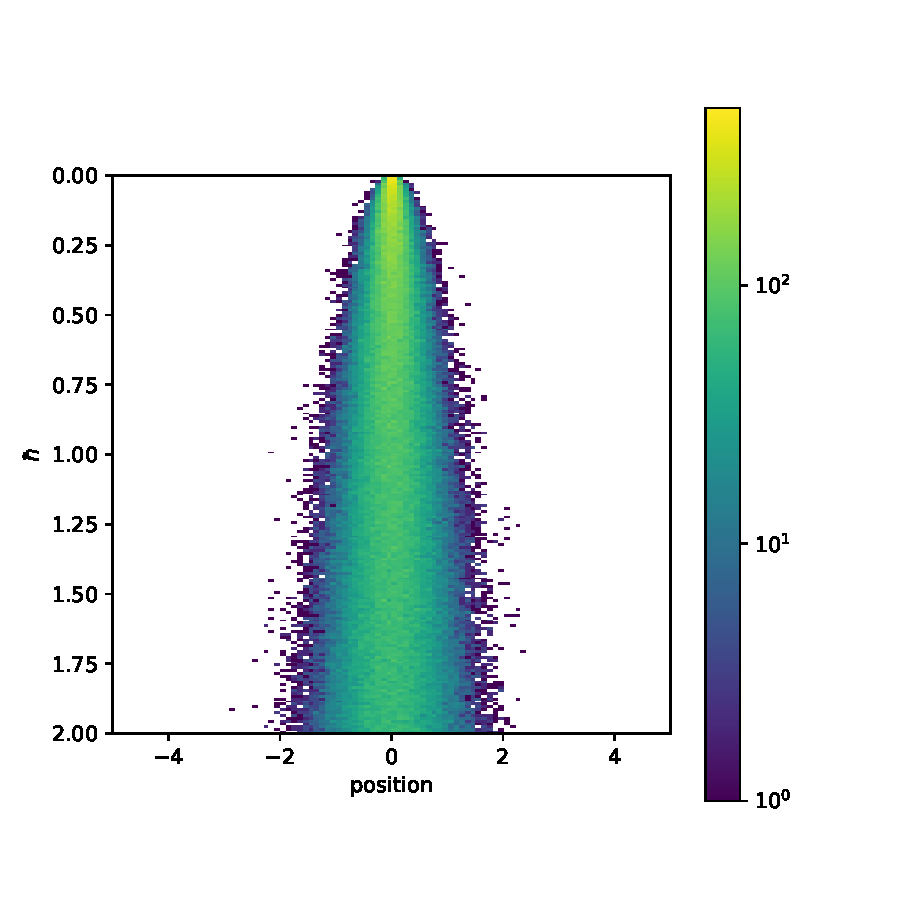
\includegraphics[width=0.6\textwidth]{../imgs/harmonic_oscillator_classical_limit/harmonic_oscillator_10_classical_limit.pdf}
			\caption{Classical limit of the harmonic oscillator.}
			\label{fig:harmonic_oscillator_classical_limit}
		\end{figure}
		In figure \ref{fig:harmonic_oscillator_classical_limit} the data is shown, generated for a particle with mass $m = 0.25$, $\mu = 10$, $\tau = 0.1$ on a time lattice with 1000 positions and 1000 Metropolis iterations.
		The parameter $\hbar$ has been varied in the range 0 to 2.

		The same data has been generated for the anharmonic oscillator.
		\begin{figure}[H]
			\centering
				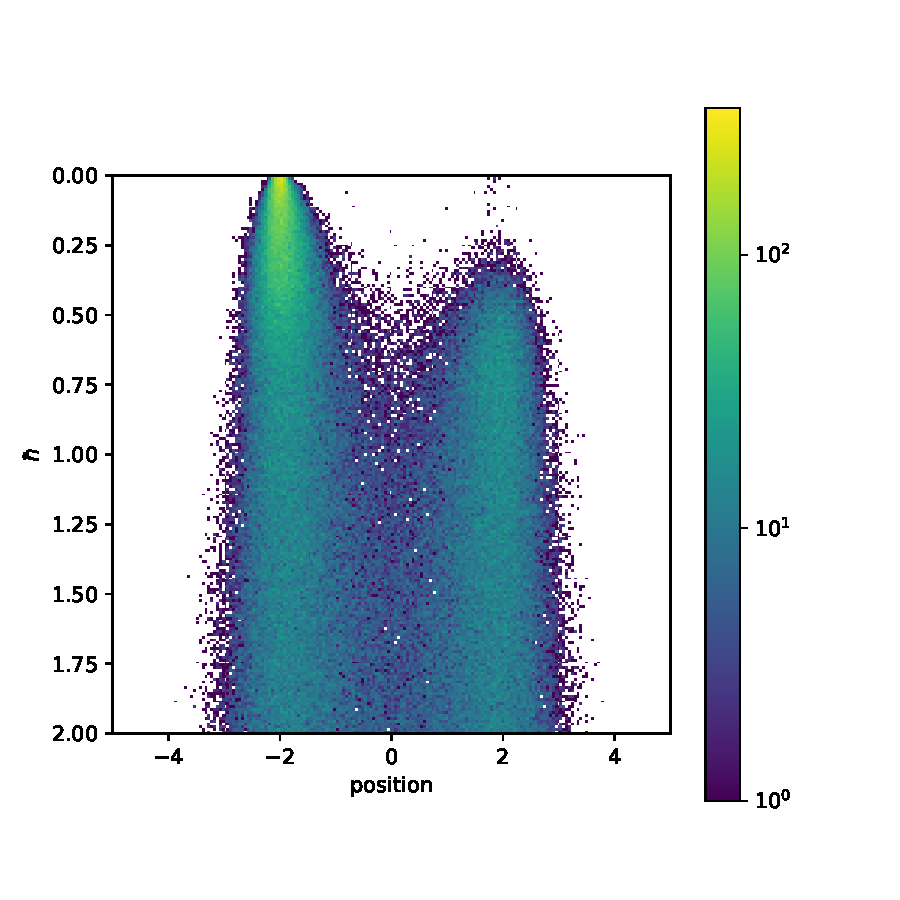
\includegraphics[width=0.6\textwidth]{../imgs/anharmonic_oscillator_classical_limit/anharmonic_oscillator_classical_limit.pdf}
			\caption{Classical limit of the anharmonic oscillator.}
			\label{fig:anharmonic_oscillator_classical_limit}
		\end{figure}
		In figure \ref{fig:anharmonic_oscillator_classical_limit} the following parameters have been used: $i = 200$, $N = 1000$, $m = 0.01$, $\mu = -10.0$, $\tau = 0.1$, $\lambda = -0.125$, corresponding to a position of the minima at $\pm 2.0$.
		The parameter range for the Heisenberg parameter is the same as for the harmonic oscillator.
		The initial state has been prepared into the left minimum.

	\subsubsection{Probability density}
		Another test I performed is to check the shape of the probability density of the harmonic oscillator.
		\begin{figure}[H]
			\centering
				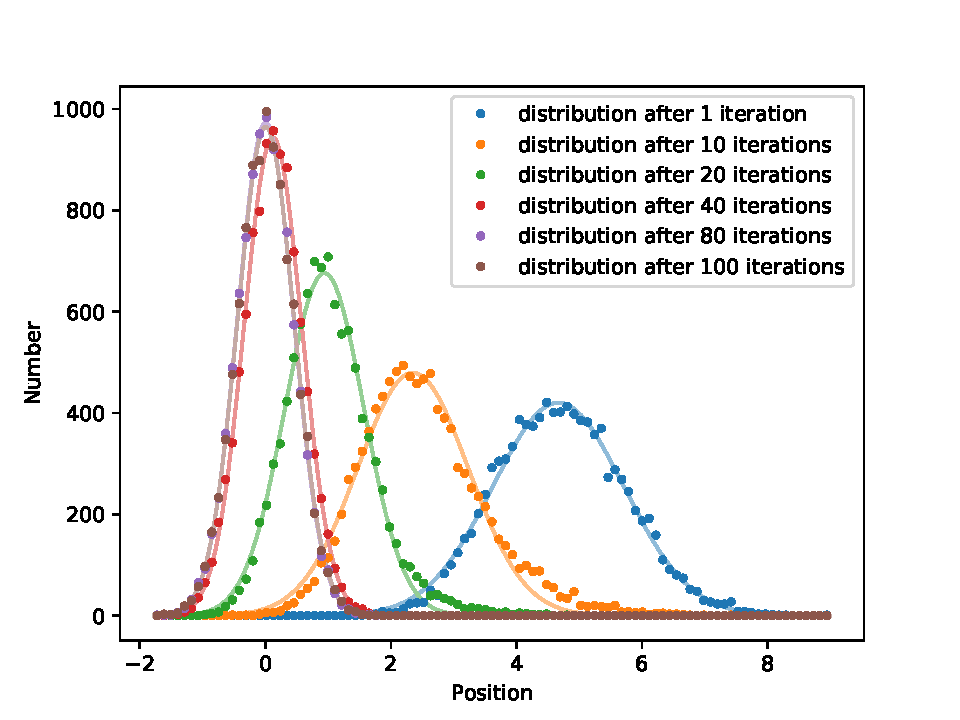
\includegraphics[width=0.6\textwidth]{../imgs/harmonic_oscillator_track/track_10010000_gauss_1_fit.pdf}
			\caption{Probability density for different Metropolis iterations of the harmonic oscillator.}
			\label{fig:harmonic_oscillator_track_10010000_gauss_1_fit}
		\end{figure}
		The parameters used for the plot in figure \ref{fig:harmonic_oscillator_track_10010000_gauss_1_fit} were $i=100$, $N=10000$, $m=0.25$, $\mu = 10.0$, $\hbar = 1$.
		The fits are gaussian distribution functions.
		\\\\
		To investigate further the probability distribution, quantile-quantile plots can be created to compare the distribution with a gaussian shape.
		\begin{figure}[H]
			\centering
			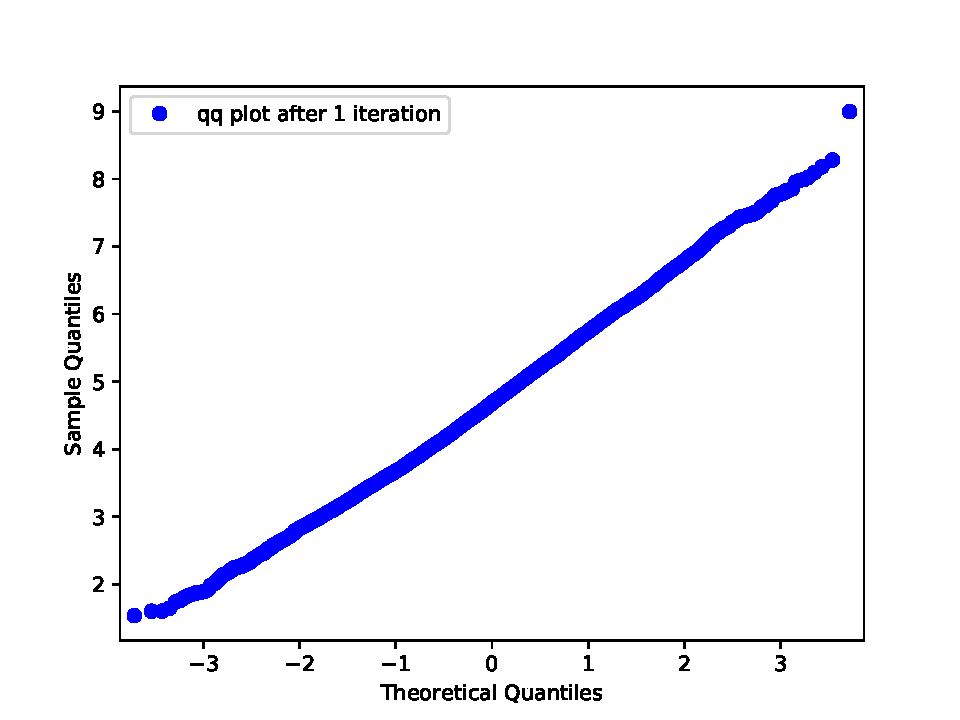
\includegraphics[width=0.4\textwidth]{../imgs/harmonic_oscillator_track/track_10010000_qq_1.pdf}
			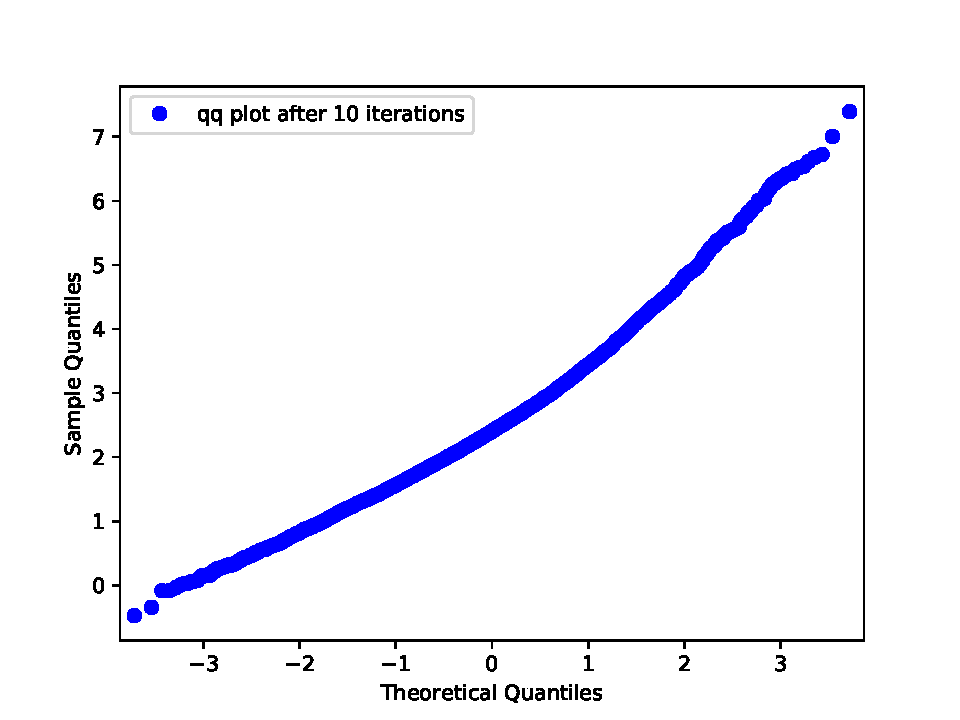
\includegraphics[width=0.4\textwidth]{../imgs/harmonic_oscillator_track/track_10010000_qq_10.pdf}
			\\
			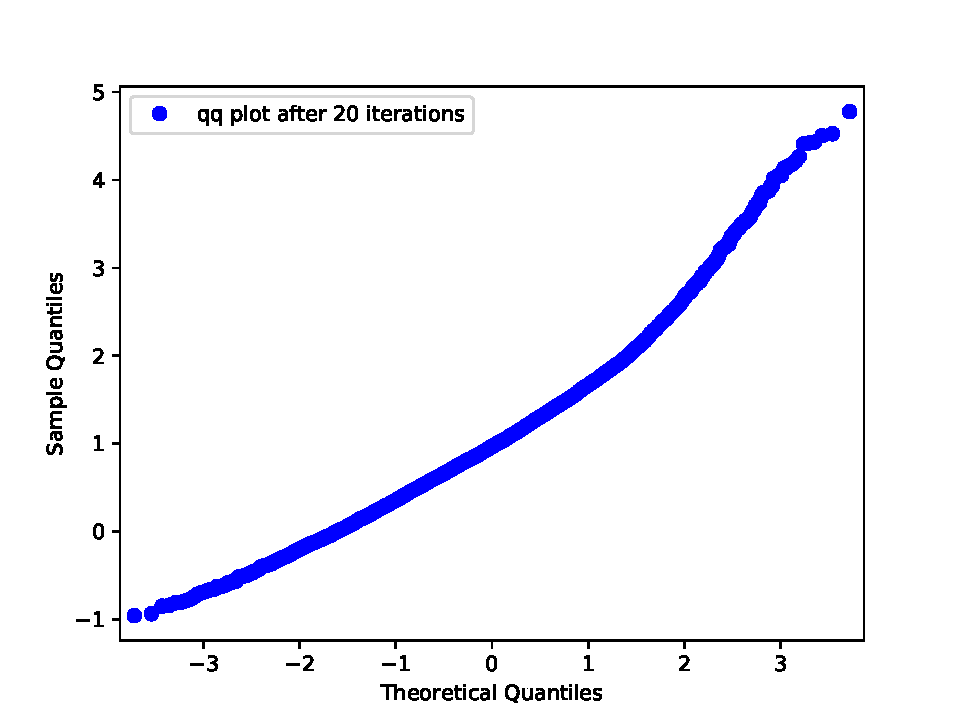
\includegraphics[width=0.4\textwidth]{../imgs/harmonic_oscillator_track/track_10010000_qq_20.pdf}
			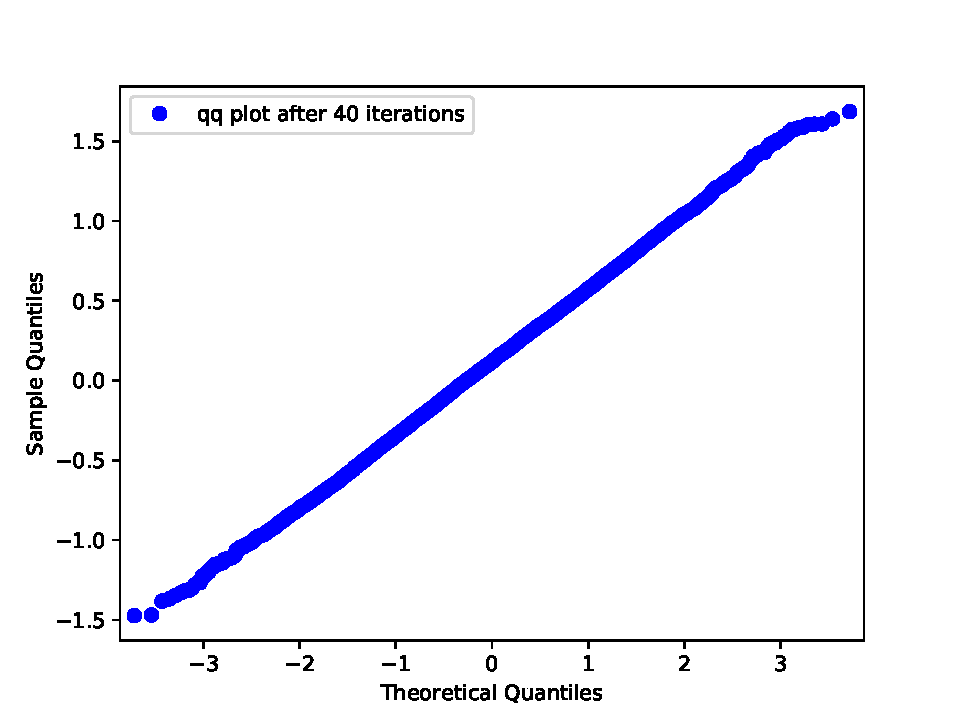
\includegraphics[width=0.4\textwidth]{../imgs/harmonic_oscillator_track/track_10010000_qq_40.pdf}
			\\
			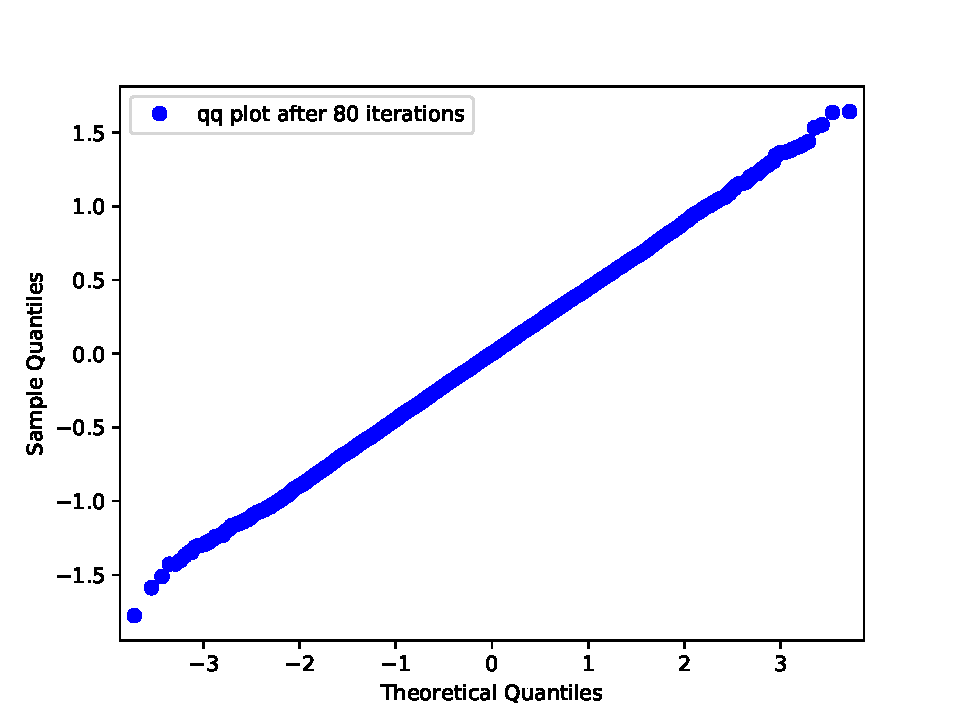
\includegraphics[width=0.4\textwidth]{../imgs/harmonic_oscillator_track/track_10010000_qq_80.pdf}
			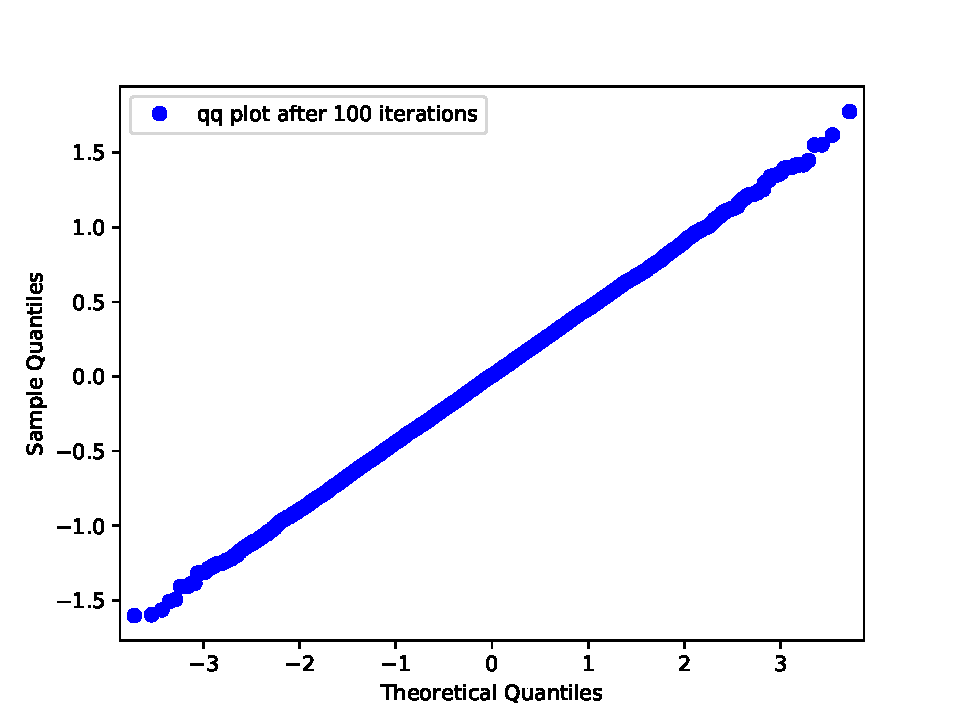
\includegraphics[width=0.4\textwidth]{../imgs/harmonic_oscillator_track/track_10010000_qq_100.pdf}
			\caption{Thermalisation of the harmonic oscillator from an exited state to the equilibrium.}
			\label{fig:harmonic_oscillator_track_track_10010000_qqs}
		\end{figure}
		In figure \ref{fig:harmonic_oscillator_track_track_10010000_qqs} quantile-quantile plots are shown for the same data and iterations as in figure \ref{fig:harmonic_oscillator_track_10010000_gauss_1_fit}.
		The experimental distribution function was compared to a gaussian distribution function.

	\subsection{Tracks}
		To visualise the behaviour of the particle I created some plots showing the track of the particle.
		\begin{figure}[H]
			\centering
				\includegraphics[width=0.6\textwidth]{../imgs/harmonic_oscillator_track/track_100100_track_100.pdf}
			\caption{Typical track of the harmonic oscillator.}
			\label{fig:harmonic_oscillator_track_100100_track_100}
		\end{figure}
		For the harmonic oscillator one gets a track similar to \ref{fig:harmonic_oscillator_track_100100_track_100}.
		The parameters used for the plot were $i=100$, $N=100$, $m=0.25$, $\mu = 10.0$, $\hbar = 1$.
		\begin{figure}[H]
			\centering
				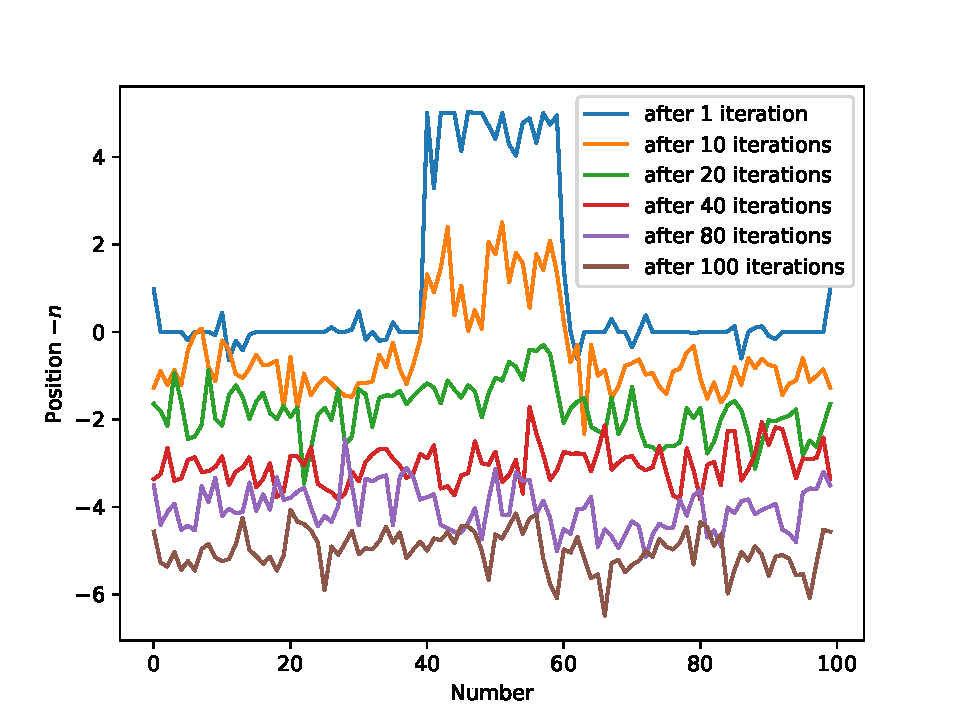
\includegraphics[width=0.6\textwidth]{../imgs/harmonic_oscillator_track/track_100100_step_track_shifted_double.pdf}
			\caption{Typical track of the harmonic oscillator, when initialised with a step function.}
			\label{fig:harmonic_oscillator_track_100100_100100_step_track_shifted_double}
		\end{figure}
		If the initial state is a step function, one gets a plot similar to \ref{fig:harmonic_oscillator_track_100100_100100_step_track_shifted_double}.
		The parameters used for the plot were $i=100$, $N=100$, $m=0.25$, $\mu = 10.0$, $\hbar = 1$.
		The individual tracks are shifted by 1 in the y direction.
		The track has been prepared with a step function with a width of 20\% in the center and a height of 5.
		\begin{figure}[H]
			\centering
				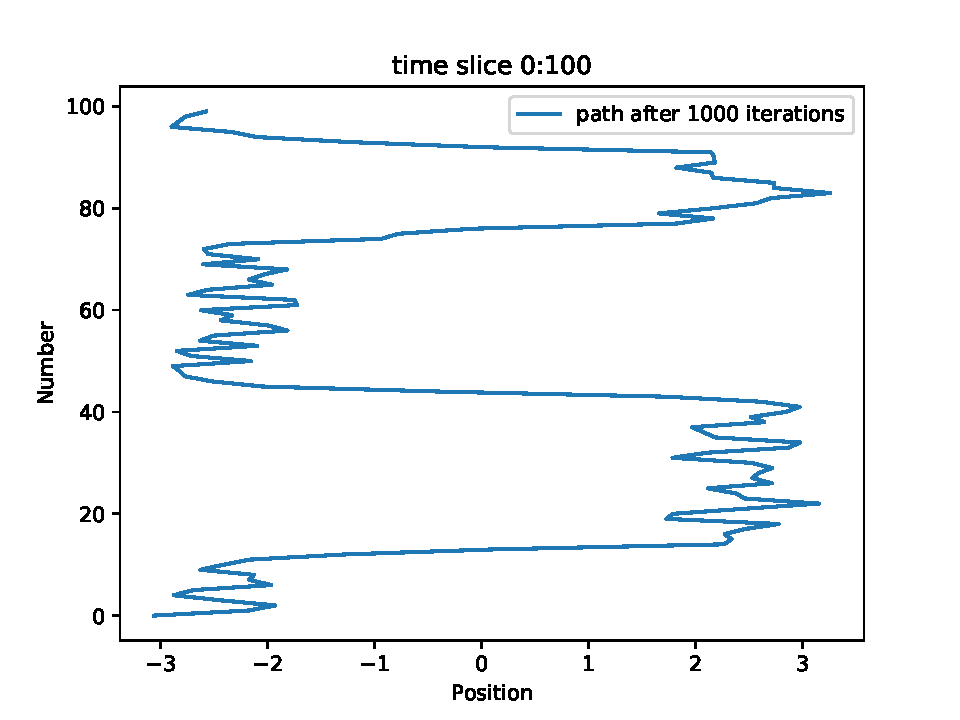
\includegraphics[width=0.6\textwidth]{../imgs/anharmonic_oscillator_track/track_100010005_track_pretty_1000.pdf}
			\caption{Typical track of the anharmonic oscillator, cut to an interesting section.}
			\label{fig:anharmonic_oscillator_track_100010005_track_pretty_1000}
		\end{figure}
		For the anharmonic oscillator one gets a track similar to the one shown in figure \ref{fig:anharmonic_oscillator_track_100010005_track_pretty_1000}.
		The parameters used for the plot were $i=1000$, $N=1000$ but cut to $N=100$, $m=0.25$, $\mu = -10.0$, $\hbar = 1$, $\lambda = -0.08$, corresponding to a position of the minima at $\pm 2.5$.

	\subsection{Measurements}
	\subsubsection{Classical limit energy}
		\begin{figure}[H]
			\centering
				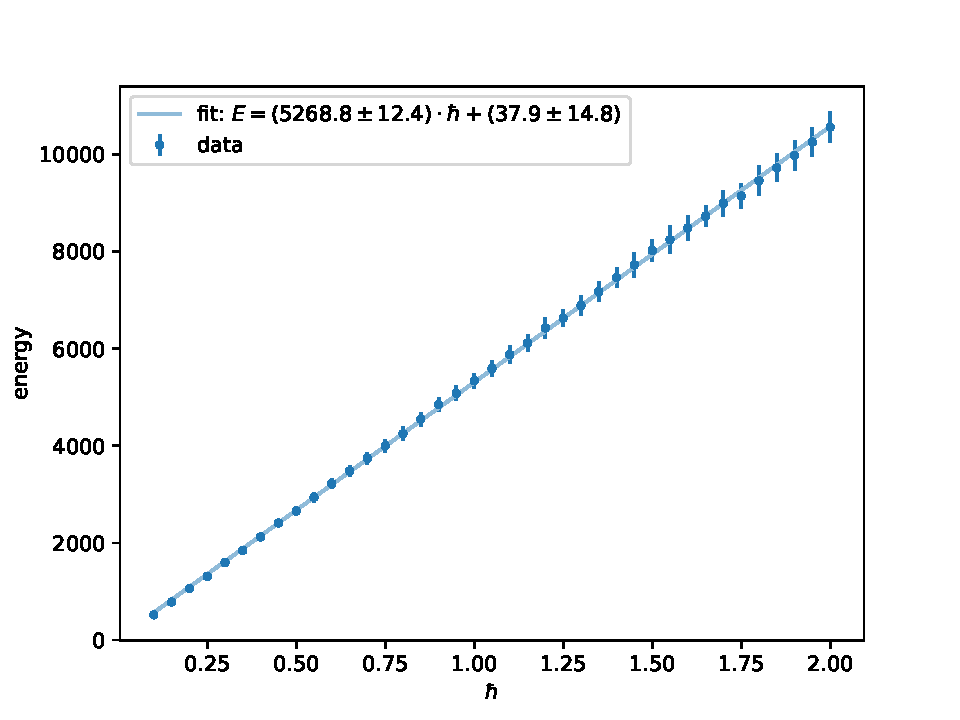
\includegraphics[width=0.6\textwidth]{../imgs/harmonic_oscillator_classical_limit_energy/harmonic_oscillator_10_classical_limit_energy.pdf}
			\caption{Classical limit energy of the harmonic oscillator.}
			\label{fig:harmonic_oscillator_classical_limit_energy}
		\end{figure}
		For plot \ref{fig:harmonic_oscillator_classical_limit_energy} the energy of the harmonic oscillator has been measured depending on the value of $\hbar$.
		The position of the thermalisation has been determined by finding the first sign change of the running mean of the slope of the energy.
		Starting from this position the integrated autocorrelation time has been calculated.
		Then the data has been blocked into blocks of at least $2 \cdot \tau_{int}$, using the upper bound of the error interval, rounded to the next higher integer, from which the energy and standard deviation of the energy has been measured.
		\\\\
		An example is shown for $\hbar = 1$ in figure \ref{fig:harmonic_oscillator_energy_measurement}.

		\begin{figure}[H]
			\centering
				\begin{subfigure}[c]{0.49\textwidth}
					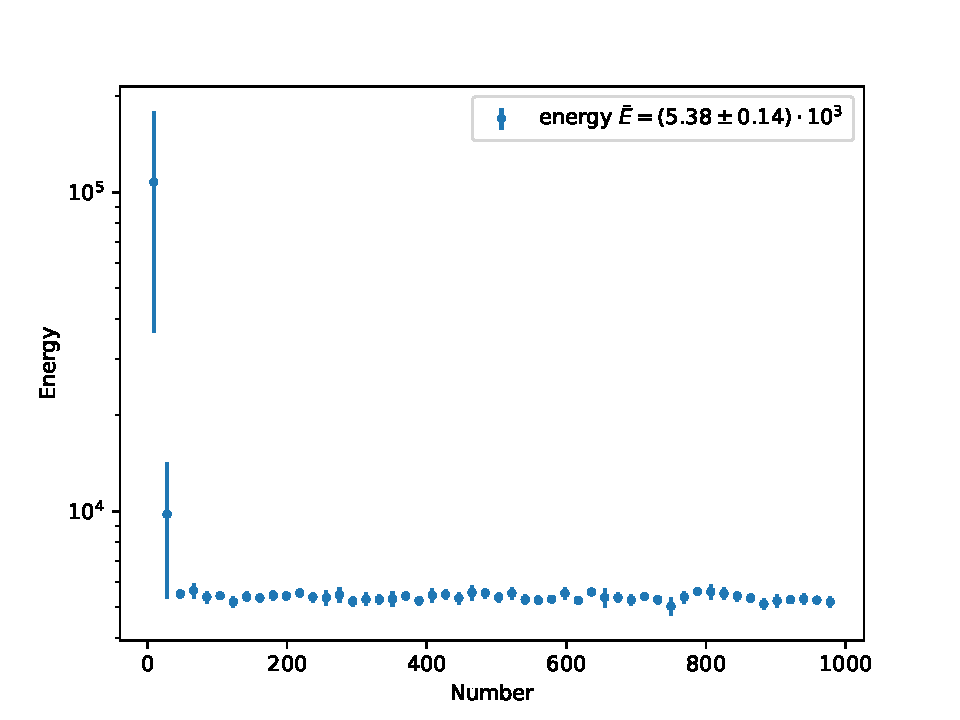
\includegraphics[width=\textwidth]{../imgs/harmonic_oscillator_track/track_10001000_thermalisation_log.pdf}
					\subcaption{Blocked energy measurements}
				\end{subfigure}
				\begin{subfigure}[c]{0.49\textwidth}
					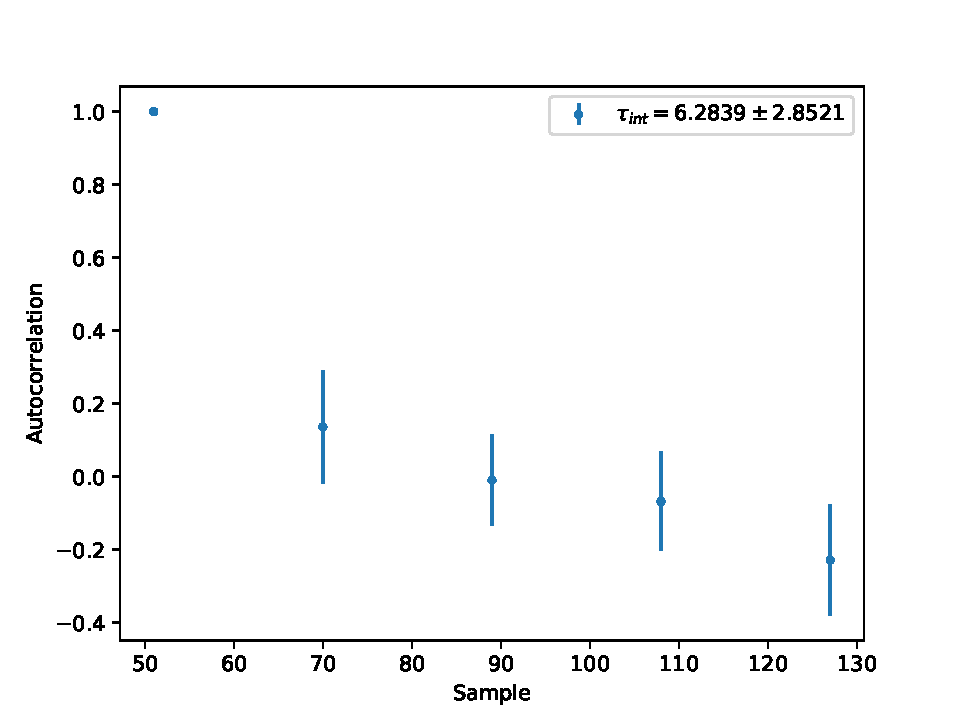
\includegraphics[width=\textwidth]{../imgs/harmonic_oscillator_track/track_10001000_thermalisation_log_autocorrelation.pdf}
					\subcaption{Autocorrelation of the enery measurements}
				\end{subfigure}
			\caption{Measurement of the energy: thermalisation and autocorrelation.}
			\label{fig:harmonic_oscillator_energy_measurement}
		\end{figure}


	\subsubsection{Tunnelling current}

	\section{Discussion}
	\subsection{Verification}
	\subsubsection{Classical limit}
		As shown in figure \ref{fig:harmonic_oscillator_classical_limit}, for $\hbar \rightarrow 0$ the probability density collapses into the minimum of the potential, as one would expect from the classical ground state.
		As visible in figure \ref{fig:anharmonic_oscillator_classical_limit}, the behaviour is similar to the harmonic oscillator, such that in the classical limit the probability density only has a significant contribution near the minima of the potential.
		Additionally one observes that there is no significant contribution on the right minimum for $\hbar < 0.3$.
		This is the behaviour one would expect:
		A classical particle in the ground state in potentials used here should state at one of the minima.
		Additionally one would expect that the probability for tunnelling tends to zero, which is observable too.

	\subsubsection{Probability density}
		As shown in figure \ref{fig:harmonic_oscillator_track_10010000_gauss_1_fit}, the initial setup was a gaussian shape, centered around the value 5 with a width of 1, visible in the blue curve.
		This corresponds to an exited state, which then thermalises into the ground state.
		The minimum of the potential is centered around 0.
		The distribution then moves towards this minimum, leading to a deviation from the gaussian shape for iterations 10 and 20.
		After 40 iterations the distribution has nearly reached the center of the potential and the distribution becomes again gaussian shaped.
		The difference between iterations 80 and 100 is negligible, this indicates that the thermalisation of the center of mass is done after 80 metropolis iterations.
		From theory one would expect the probability density to be gaussian shaped in the ground state.
		\\\\
		As previously mentioned, one can confirm that the initial setups is a gaussian distribution with center 5 and width 1.
		In the qq-plots for iterations 10 and 20 the deviation from a straight line is claerly visible.
		After the 40th iteration, the center of the distribution has reached 0 and the qq plot matches a straight line, corresponding to a gaussian distribution.
		\\\\
		From these verifications I am confident, that my code is correct.

	\subsection{Tracks}
		%TODO missing harmonic, anharmonic tracks
		In figure \ref{fig:harmonic_oscillator_track_100100_100100_step_track_shifted_double} one can see how the step function vanishes with increasing Metropolis iteration number.
		The step function disappeared after around 40 Metropolis iterations.
		In figure \ref{fig:anharmonic_oscillator_track_100010005_track_pretty_1000} one sees a part of the anharmonic oscillator track.
		One can clearly see the instants of time when a tunnelling event occurs.

	\subsection{Measurements}
	\subsubsection{Classical limit energy}

	\subsubsection{Tunnelling current}

	\section{Summary and Outlook}
	\newpage
	\begin{thebibliography}{widestlabel}
		\bibitem{github} Public Github repository: Harmonic Oscillator, Benedikt Otto (s6beotto), \\\url{https://github.com/s6beotto/Harmonic-Oscillator}.
		\bibitem{latexrun} Public Github repository: latexrun, Austin Clements (aclements), \\\url{https://github.com/aclements/latexrun}.
		\bibitem{creutz_freedman} M. Creutz and B. Freedman, \textit{A statistical approach to quantum mechanics}, Annals of Physics, \textbf{132}, 427-462 (1981).
		\bibitem{rodgers_raes} R. Rodgers and L. Raes, \textit{Monte Carlo simulations of harmonic and anharmonic oscillators in discrete Euclidean time}, DESY Summer Student Programme (2014).
	\end{thebibliography}
	\appendix
	\section{Directory structure}

	\subsection{Data generation}
	\begin{figure}[H]
		\centering
		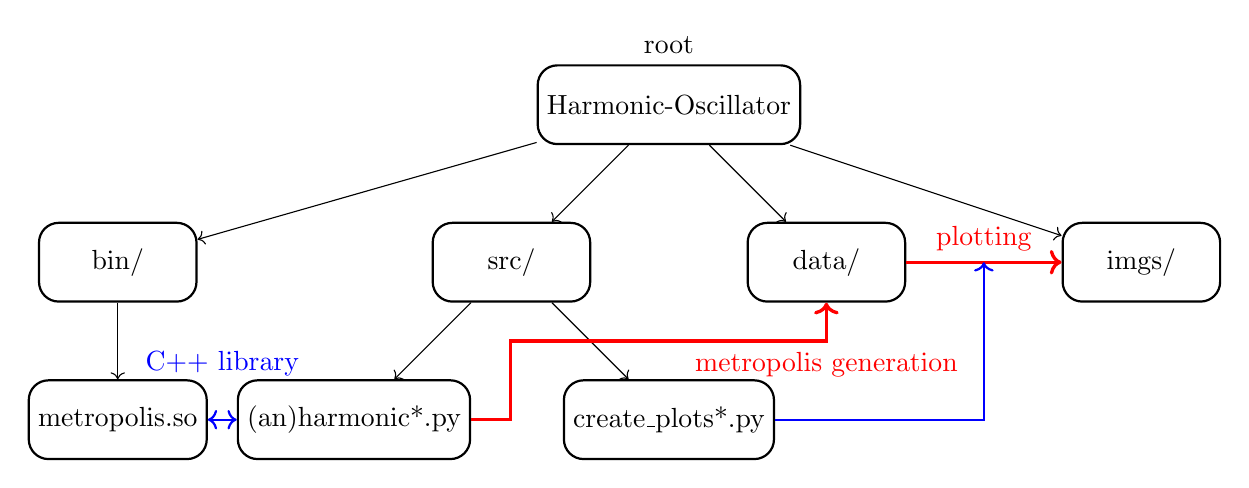
\begin{tikzpicture}
		\draw[color=black, thick]
		node[draw,minimum width=2cm,minimum height=1cm,label=root,rounded corners=0.25cm] (root) at (0, 0){Harmonic-Oscillator}
		node[draw,minimum width=2cm,minimum height=1cm,rounded corners=0.25cm] (bin) at (-7, -2){bin/}
		node[draw,minimum width=2cm,minimum height=1cm,rounded corners=0.25cm] (bin_metropolis) at (-7, -4){metropolis.so}
		node[draw,minimum width=2cm,minimum height=1cm,rounded corners=0.25cm] (src) at (-2, -2){src/}
		node[draw,minimum width=2cm,minimum height=1cm,rounded corners=0.25cm] (src_create) at (-4, -4){(an)harmonic*.py}
		node[draw,minimum width=2cm,minimum height=1cm,rounded corners=0.25cm] (src_plot) at (0, -4){create\_plots*.py}
		node[draw,minimum width=2cm,minimum height=1cm,rounded corners=0.25cm] (data) at (2, -2){data/}
		node[draw,minimum width=2cm,minimum height=1cm,rounded corners=0.25cm] (imgs) at (6, -2){imgs/};
		\draw [->] (root) -- (bin);
			\draw [->] (bin) -- (bin_metropolis);
		\draw [->] (root) -- (src);
			\draw [->] (src) -- (src_create);
			\draw [->] (src) -- (src_plot);
		\draw [->] (root) -- (data);
		\draw [->] (root) -- (imgs);
		\draw [<->, thick, blue] (bin_metropolis) -- (src_create) node[midway,above=12] {C++ library};
		\draw [->, very thick, red] (src_create.east) -| ++(0.5, 1) -| (data) node[midway,below] {metropolis generation};
		\draw [->, very thick, red] (data) -- (imgs) node[midway,above] {plotting};
		\draw [->, thick, blue] (src_plot.east) -| (4, -2);
		\end{tikzpicture}
		\caption{Directory structure of the project for data generation.}
		\label{fig:scheme_dirs_data_generation}
	\end{figure}

	\subsection{Report generation}
	\begin{figure}[H]
		\centering
		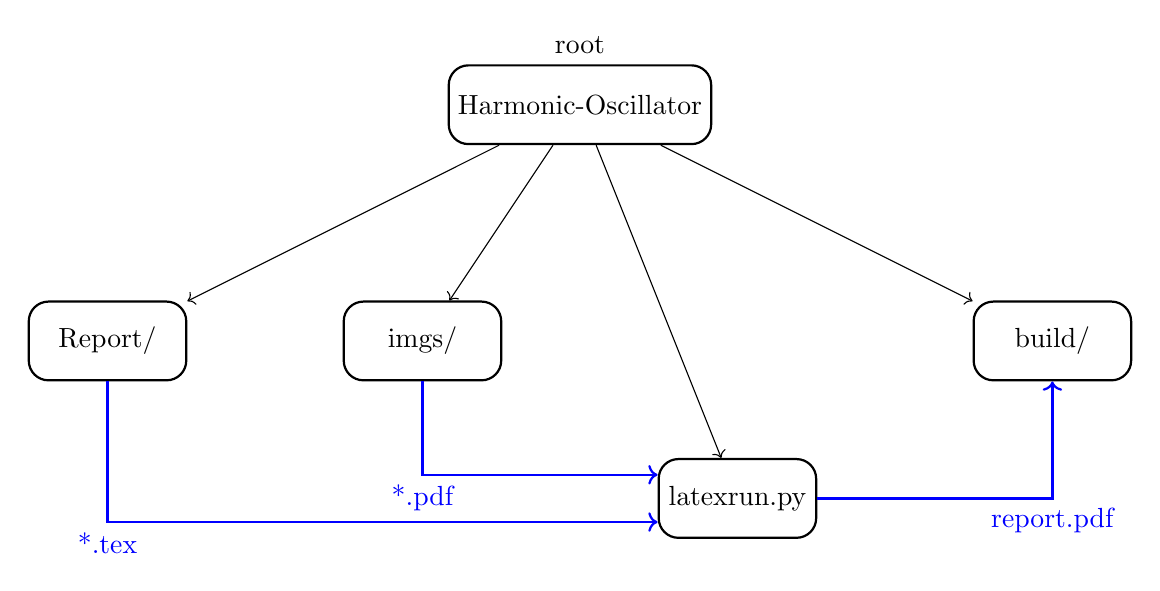
\begin{tikzpicture}
		\draw[color=black, thick]
		node[draw,minimum width=2cm,minimum height=1cm,label=root,rounded corners=0.25cm] (root) at (0, 0){Harmonic-Oscillator}
		node[draw,minimum width=2cm,minimum height=1cm,rounded corners=0.25cm] (report) at   (-6,  -3){Report/}
		node[draw,minimum width=2cm,minimum height=1cm,rounded corners=0.25cm] (imgs) at     (-2, -3){imgs/}
		node[draw,minimum width=2cm,minimum height=1cm,rounded corners=0.25cm] (latexrun) at (2,  -5){latexrun.py}
		node[draw,minimum width=2cm,minimum height=1cm,rounded corners=0.25cm] (build) at    (6,  -3){build/};
		\draw [->] (root) -- (report);
		\draw [->] (root) -- (imgs);
		\draw [->] (root) -- (latexrun);
		\draw [->] (root) -- (build);
		\draw [<-, thick, blue] (latexrun.west) + (0,-3mm) -| (report.south) node[midway,below] {*.tex};
		\draw [<-, thick, blue] (latexrun.west) + (0, 3mm) -| (imgs.south)   node[midway,below] {*.pdf};
		\draw [->, thick, blue] (latexrun) -| (build.south)                  node[midway,below] {report.pdf};
		\end{tikzpicture}
		\caption{Directory structure of the project for report generation.}
		\label{fig:scheme_dirs_report_generation}
	\end{figure}
	The file \verb!latexrun.py! is taken from \cite{latexrun}.
\end{document}